\documentclass[10pt,a4paper]{article}
\newcommand{\judul}{Modul Bunyi}
\newcommand{\penulis}{bintangpelajar.com}
\usepackage[latin1]{inputenc}
\usepackage{amsmath}
\usepackage{microtype}
\usepackage[none]{hyphenat}
\usepackage{verbatim}
\usepackage{amsfonts}
\usepackage{amssymb}
\usepackage{enumitem}
\renewcommand{\familydefault}{\sfdefault}
\usepackage{mathpazo}
\renewcommand{\rmdefault}{put}
\usepackage{enumitem}
\usepackage[dvipsnames,svgnames]{xcolor}
\usepackage{tkz-euclide}
\usetkzobj{all}
\usepackage{graphicx}
\usepackage{fancyhdr}
\usepackage{tikz} 	
\usepackage{adjustbox}
\usepackage{multicol}
\usepackage{lipsum}
\usepackage[headsep=0.2cm,footskip=2pt,left=0.3cm,right=0.7cm,top=1.7cm,bottom=1.0cm]{geometry}
\usepackage{cancel} \usepackage{xcolor}
\usepackage{tcolorbox}
\usetikzlibrary{decorations.pathmorphing,patterns}
\usetikzlibrary{decorations.pathreplacing,calc}
 \newcommand\coret[2][red]{\renewcommand\CancelColor{\color{#1}}\cancel{#2}}
\SetLabelAlign{Center}{\hfil\makebox[1.0em]{#1}\hfil}

\newtcolorbox{mybox}[1][] { colframe = blue!10, colback = blue!3,boxsep=0pt,left=0.2em, coltitle = blue!20!black, title = \textbf{jawab}, #1, } 

%---------- kunci (jika 1 ) muncul
\def\tampilkunci{1}
\newcommand{\hide}[1]{\ifnum\tampilkunci=1
%
\begin{mybox}
 #1
\end{mybox}
%
\vspace{\baselineskip}\fi}

\newcommand*\cicled[1]{\tikz[baseline=(char.base)]{\node[white, shape=circle, fill=red!80,draw,inner sep=0.5pt](char){#1};}}

\newcommand*\kunci[1]{\ifnum\tampilkunci=1
%
\tikz[baseline=(char.base)]{\node[red, shape=circle,draw,inner sep=0.5pt,xshift=2pt](char){#1};}\stepcounter{enumii}
\fi\ifnum\tampilkunci=0
%
\hspace{3pt}#1\stepcounter{enumii}
%
\fi}

%------------- MULAI FUNGSIKU ------------
\newcommand{\cartesius}[3]{
\draw[help lines] (-1,-1) grid (#1);
\foreach \x in {1,2,...,#2}{
\node at (\x,0)[scale=0.5]{\x};}
\foreach \y in {1,2,...,#3}{
\node at (0,\y) [scale=0.5]{\y};}}

\newcommand{\pers}[1]{\begin{align*} #1 \end{align*}}
% \sci{ }  misal  x 10^2  tinggal tulis 
% \sci{2} 
\newcommand{\sci}[1]{$\times 10^{#1}$}

\newcommand{\scip}[1]{\times 10^{#1}}

%----membuat tanda silang di samping text
\newcommand*\silang[1]{\tikz[baseline=(char.base)]{
\draw[red,thick](-0.2,-0.20)--(0.2,0.2);
\draw[red,thick](-0.2,0.20)--(0.2,-0.2);
\node[black](char){#1};
}}
%----- membuat tanda centang di mana saja
\newcommand*\centang[1]{\tikz[baseline=(char.base)]{
\draw[red, very thick](-0.2,0.1)--(-0.1,0)--(0.2,0.3);
\node(char){#1};
}}
%------------mewarnai text merah
\newcommand*\merah[1]{
\textcolor{red}{#1}}
\newcommand*\pilgan[1]{
\begin{enumerate}[label=\Alph*., itemsep=0pt,topsep=0pt,leftmargin=*,align=Center] #1 
\end{enumerate}}

%---- membuat pernyataan pada soal SBMPTN
\newcommand*\pernyataan[1]{
\begin{enumerate}[label=(\arabic*), itemsep=0pt,topsep=0pt,leftmargin=*] #1 
\end{enumerate}}

%------ lebar baris pada tabular
\newcommand{\baris}[1]{\renewcommand\arraystretch{#1} }
%\newcommand{\tabel}[2j]{\begin{tabular}{#1}
%\end{tabular}
%------------ END OF FUNGSIKU ----------- 





%--------------- begin{document}-----------
\pagestyle{fancy}
\fancyhf{} 
\rhead{\penulis}
\lhead{\judul}
\rfoot{Hal \thepage}
\begin{document}


\begin{multicols*} {3} 
\begin{enumerate}[itemsep=0mm]

%------------ nomor 1----------
\item \pernyataan{
\item Bunyi di udara merupakan gelombang longitudinal
\item Bunyi merupakan gelombang mekanik 
\item Bunyi merambat memerlukan zat perantara 
}
Pernyataan di atas yang benar adalah . . . .
\pilgan{
\item 1) dan 2)
\item 1) dan 3)
\item 2) dan 3)
\item [\kunci{D.}] 1), 2), da 3)
\item 3) saja
}

%---------- nomor 2 ---------
\item Kedua buah sumber bunyi pada gambar di bawah bergetar secara koheren. Kenyaringan di dengar di P bila $r_1 = r_2$. Dengan menaikkan secara perlahan $r_1$, bunyi terlemah didengar ketika $r_1 - r_2$ adalah 20 cm, 60 cm, dan 100 cm. Jika laju rambat bunyi 340 m/s, maka besar frekuensi sumber bunyi adalah . . . 

\pilgan{
\item 136 Hz
\item 475 Hz
\item 680 Hz
\item 850 Hz
\item 1700 Hz
}

%--------- nomor 3 ---------
\item Tali yang panjangnya 5 m bertegangan 2 N dan digetarkan sehingga terbentuk gelombang stationer. Jika massa tali 6,25 $\times 10^{-3}$ kg, maka cepat rambat gelombang di tali adalah . . . . m/s
\pilgan{
\item 2
\item 5
\item 6 
\item 10
\item 40
}


%--------- nomor 4 ------------ 
\item Pada suhu tertentu modulus bulk air adalah 1,96 $\times 10^9$ N/m$^2$ dan massa jenisnya $10^3$ kg/m$^3$. Maka kecepeatan perambatan gelombang bunyi di dalam air adalah . . . .
\pilgan{
\item 1,2 $\times 10^3$
\item 1,4 $\times 10^3$
\item 1,6 $\times 10^3$
\item 1,8 $\times 10^3$
\item 2,0 \sci{3}
}


%---------- nomor 5 --------------
\item Kecepatan rambat bunyi dalam gas hidrogen pada suhu 250 K adalah 1350 m/s. Jika tetapan Laplace hidrogen dan oksigen dianggap sama, berapa cepat rambat bunyi dalam oksigen pada suhu 360 K?
\pilgan{
\item 2700 m/s
\item 1505 m/s
\item 1350 m/s \item 675 m/s \item 405 m/s }

%-------- nomor 6 -------------
\item Seutas kawat tembaga ($\rho$ = 8,9 g/cm$^3$) diikat pada salah satu ujung lainnya dihubungkan dengan sebuah benda tergantung (m = 10 kg). Maka frekuensi nada dasar yang dihasilkan, jika panjang kawat 50 cm dan luas penampang kawat 0,5 mm$^2$ adalah . . . 
\pilgan{
\item 110 Hz
\item 120 Hz
\item 130 Hz
\item 140 Hz
\item [\kunci{E.}]150 Hz
}
\hide{
\baris{1}
\begin{tabular}{ll}
\multicolumn{2}{l}{$\rho$ = 8,9 g/cm$^3$ = 8900 kg/m$^3$ } \\
$F$ = 100 N & $l$ = 0,5 m  \\
\multicolumn{2}{l}{$A$ = 0,5 mm$^2$= 0,5 \sci{-7} m$^2$ } \\
\multicolumn{2}{l}{ditanya :  $f$ = . . . .?} \\ 
\end{tabular}
\pers{
v&=\sqrt{\frac{Fl}{m}}\\
v&=\sqrt{\frac{100.0,5}{\scip{-23}}}
}
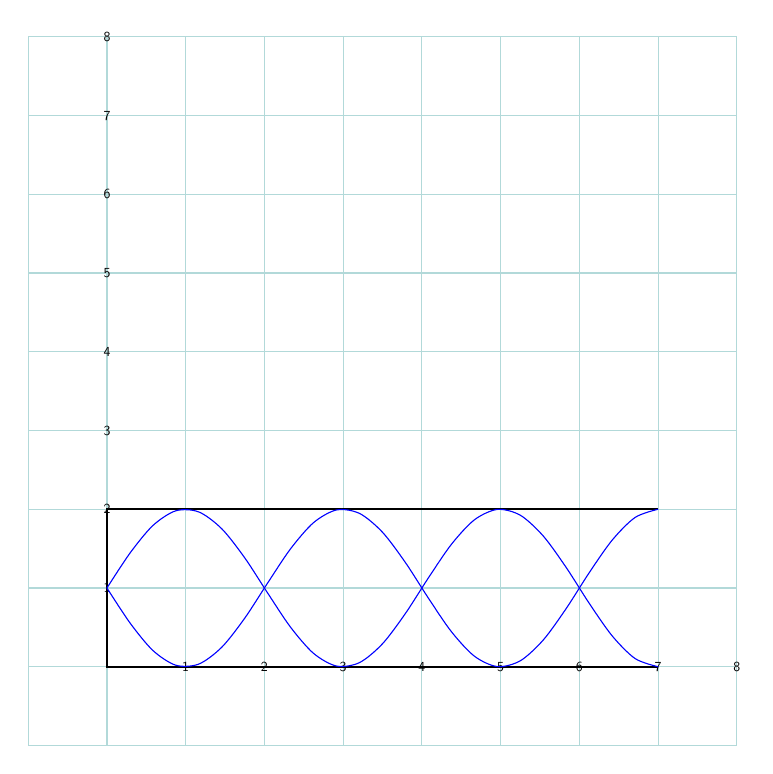
\begin{tikzpicture}
\cartesius{8,8}{8}{8}
\draw[thick] (7,0)--(0,0)--(0,2)--(7,2);
%\foreach [evaluate={\y=sin(\x*pi r)}] \x in {0,0.1,...,7}{
%\draw(\x,\y) circle(0.01cm);}
 \draw[domain=0:7,smooth,variable=\x,blue] plot ({\x},{sin(\x*pi/2 r)+1});
\draw[domain=0:7, smooth, variable=\x,blue]plot ({\x},{-sin(\x*pi/2 r)+1});
\end{tikzpicture}
}
 \end{enumerate} 
 \end{multicols*} \vspace{1cm} %-------------------------------------------




\setlength{\columnsep}{0pt}
\vspace{0.15cm}



\begin{tabular} {|c|c|c|c|c|c|c|c|}
\hline
no & jwb & no & jwb & no & jwb & no & jwb \\ \hline
1 &B  & 11 &A  & 21 &C  & 31&F \\ \hline
2 &D  & 12 &A  & 22 &D  & 32&D  \\ \hline
3 &C  & 13 &B  & 23 &A  & 33&B \\ \hline
4 &D  & 14 &D  & 24 &A  & 34&C \\ \hline
5 &B  & 15 &D  & 25 &E  & 35&B \\ \hline
6 &B  & 16 &C  & 26 &A  & 36&E \\ \hline
7 &E  & 17 &A  & 27 &C  & 37&A \\ \hline
8 &E  & 18 &C  & 28 &E  & 38&A \\ \hline
9 &C  & 19 &B  & 29 &E  & 39&E \\ \hline
10 &B  & 20 & F & 30 & E & 40&D \\ \hline


\end{tabular}

 \end{document}
